%%%%%%%%%%%%%%%%%%%%%%%%%%%%%%%%%%%%%%%%%%%%%%%%%%%%%%%%%%%

\section{Apresentação dos dados}

O problema de classificação com o reconhecimento de atividades humanas utiliza como base de dados amostras tomadas do acelerômetro e do giroscópio do \textit{smartphone} preso à cintura do candidato. Dessa forma, com base na leitura desses sensores, pode-se identificar se a pessoa está caminhando, subindo escadas, descendo escadas, sentada, de pé ou deitada, que representam as seis classes do problema.

Os dados brutos utilizados são formados da concatenação das 128 medições dos sensores de orientação e aceleração, para os eixos $x$, $y$ e $z$, em cada janela de tempo. Dessa forma, chega-se a um \textit{dataset} de treinamento e teste com 768 atributos. São um total de 7352 amostras para treinamento e validação, e 2947 amostras para teste.

Além dos dados brutos, é fornecido também os dados processados, com extração sobre os dados no tempo, na frequência, e também características estatísticas dos mesmos. Os dados tratados são formados por amostras de 561 atributos derivados da análise no tempo e na frequência dos dados provenientes do acelerômetro e do giroscópio do \textit{smartphone}. 

O balanceamento das classes nos conjuntos de dados foi realizado por meio do cálculo da taxa de ocorrência dos mesmos, dada de acordo com \eqref{eq:rate}. A \autoref{fig:balancingofclasses} mostra a distribuição das classes, e pode-se ver que não existe um balanceamento homogêneo, onde a classe 3 é a que menos ocorre, enquanto a classe  6 é a que mais ocorre.

Devido a esse desbalanceamento, a métrica que será utilizada para a avaliação do desempenho de cada classificador será a acurácia balanceada, dada por \eqref{eq:ba}.

\begin{equation}\label{eq:rate}
	Rate_i = \frac{N_i}{N}
\end{equation}

% TODO: \usepackage{graphicx} required
\begin{figure}[H]
	\centering
	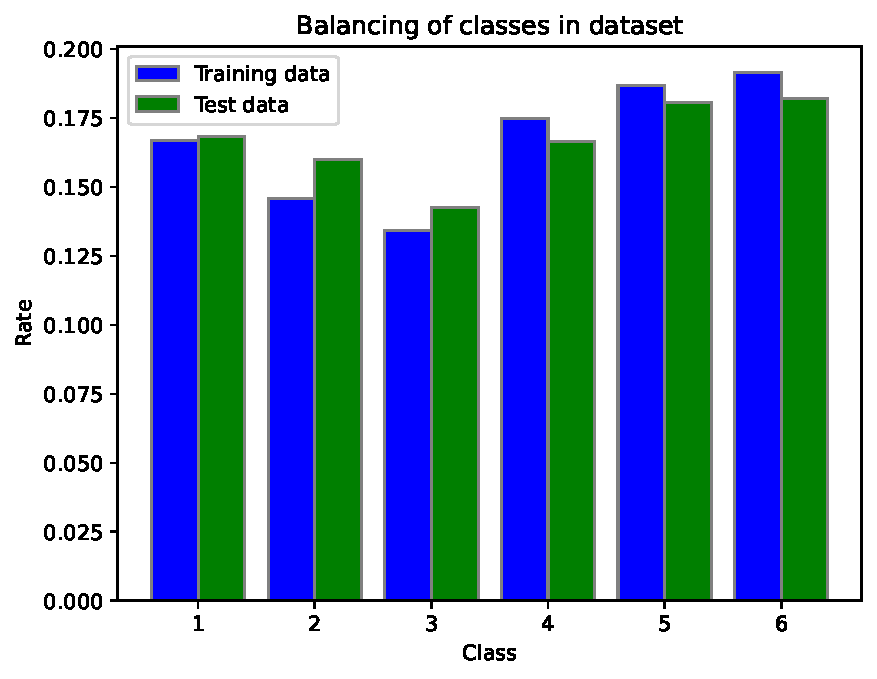
\includegraphics[width=0.55\linewidth]{../../plot/Balancing_of_classes}
	\caption{Gráfico da ocorrência das classes nos conjuntos de dados de treinamento e teste.}
	\label{fig:balancingofclasses}
\end{figure}

\begin{equation}\label{eq:ba}
	BA = \frac{\sum_{i=1}^{Q}Recall_i}{Q} = \frac{\sum_{i=1}^{Q}\frac{\text{TP}_i}{N_i}}{Q} = \frac{\sum_{i=1}^{Q}\frac{\text{TP}_i}{N\cdot Rate_i}}{Q}
\end{equation}



%%%%%%%%%%%%%%%%%%%%%%%%%%%%%%%%%%%%%%%%%%%%%%%%%%%%%%%%%%%
\clearpage
\section{Classificação via Regressão Logística}

A classificação multi-classe é feita de forma elegante ao ter um modelo, que dadas $Q$ classes à serem reconhecidas, apresente $Q$ saídas, onde cada saída é a probabilidade da amostra pertencer à classe em questão. Tal implementação se dá por meio da função \textit{softmax}, enunciada em \eqref{eq:softmax}, e a saída é dada pela notação \textit{one-hot encoding}.

\begin{equation}\label{eq:softmax}
	\hat{y}_k (\+x(i)) = \frac{e^{\left(\+\Phi(\+x(i))^T\+w_k\right)}}{\sum_{j}e^{\left(\+\Phi(\+x(i))^T\+w_j\right)}}
\end{equation}

Onde o $\+w_k$ é o vetor de pesos para a classe $k$, e a matriz de pesos $\+W$ é dada por \eqref{eq:W}.

\begin{equation}\label{eq:W}
	\+W = \begin{bmatrix}
		\+w_1 \\
		\+w_2 \\
		\vdots \\
		\+w_Q
	\end{bmatrix}
\end{equation}

Não existe forma fechada para a obtenção dos pesos de $\+W$, logo, o mesmo precisa ser feito de forma iterativa. A métrica utilizada como função de custo para o problema é a entropia cruzada, dada por \eqref{eq:JCE}. O otimização dos pesos se dá pela técnica do gradiente descendente, dado por \eqref{eq:dJCE}.

\begin{equation}\label{eq:JCE}
	J_{CE}(\+W) = -\sum_{i=0}^{N-1}\sum_{k=1}^{Q}y_{i,k}\log\left[\hat{y}_k(\+x(i)\right]
\end{equation}

\begin{equation}\label{eq:dJCE}
	\frac{\partial J_{CE}(\+W)}{\partial \+w_k} = \sum_{i=0}^{N-1} \left(y_{i,k} - \hat{y}_k\left(\+x(i)\right)\right)\+\Phi(\+x(i))^T
\end{equation}

A atualização dos pesos é dada por \eqref{eq:wk1}, onde $l$ é a iteração dos pesos.

\begin{equation}\label{eq:wk1}
	\+W[l+1] = \+W[l] - \eta\nabla\+W
\end{equation}

Devido ao tamanho do conjunto de dados, foi proposto o treinamento por \textit{mini-batch}, testadas com tamanhos de 500, 1000 e 2000 amostras, e um passo ($\eta$) de 0,01, que apresentou boa convergência nos testes realizados \textit{a priori}. O processo de validação cruzada para o treinamento do modelo foi feito na forma \textit{holdout}, considerando o conjunto de validação 30\% do \textit{dataset} de treinamento. A inicialização dos pesos foi feita de forma aleatória, seguindo uma distribuição gaussiana, nos entornos de 0.



%%%%%%%%%%%%%%%%%%%%%%%%%%%%%%%%%%%%%%%%%%%%%%%%%%%%%%%%%%%
\clearpage
\subsection{Dados tratados}

\subsubsection*{\textit{Mini-batch} 500 amostras}

Para um primeiro caso, treinou-se o modelo de regressão logística utilizando o \textit{mini-batch} de 500 amostras. A cada 500 amostras de treinamento, entregues em ordem aleatória a cada época, realiza-se a evolução da matriz de pesos $\+W$, calculando a nova função de custo (entropia cruzada), e o valor da acurácia balanceada, para todo conjunto de treinamento e validação.

A \autoref{fig:CE_500_epochs_batch_size500} mostra o decaimento da entropia cruzada de treinamento e validação durante as épocas de treinamento. Para 500 épocas, observa-se que não há o estado de regime das métricas, ou a inversão do crescimento da entropia cruzada de validação, que indicaria \textit{overfitting}. Porém, analisando a acurácia balanceada do modelo, exibida na \autoref{fig:BA_500_epochs_batch_size500}, percebe-se que a medida de desempenho apresenta saturação, após aproximadamente 300 épocas de treinamento, sendo assim utilizada para a parada antecipada (\textit{early stopping}) do treinamento do modelo.

% TODO: \usepackage{graphicx} required
\begin{figure}[H]
	\begin{subfigure}[H]{0.49\textwidth}
		\centering
		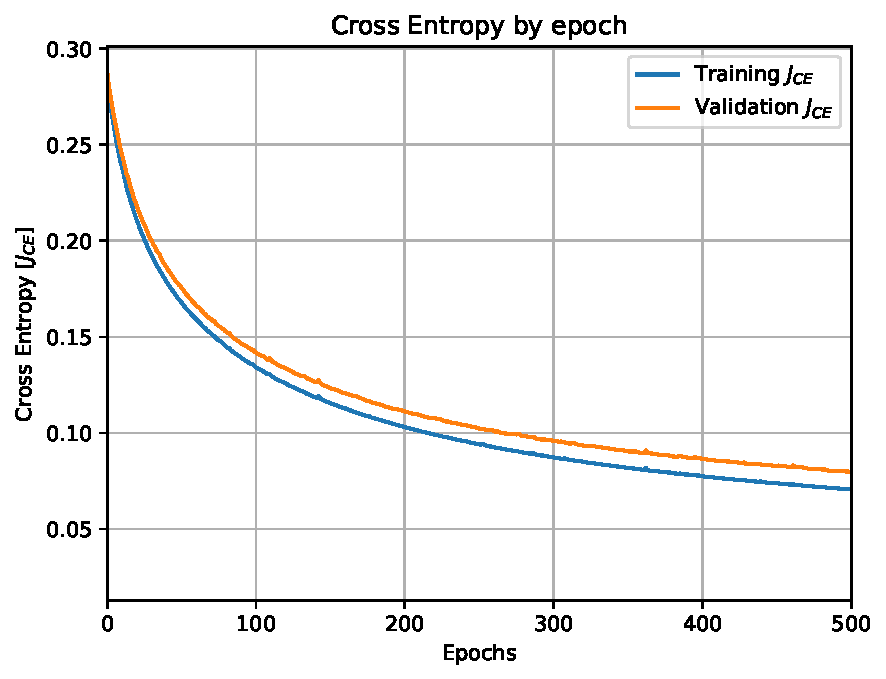
\includegraphics[width = \linewidth]{../../plot/LR_1/CE_500_epochs_batch_size500}
		\caption{Evolução da entropia cruzada.}
		\label{fig:CE_500_epochs_batch_size500}
	\end{subfigure}
	\begin{subfigure}[H]{0.49\textwidth}
		\centering
		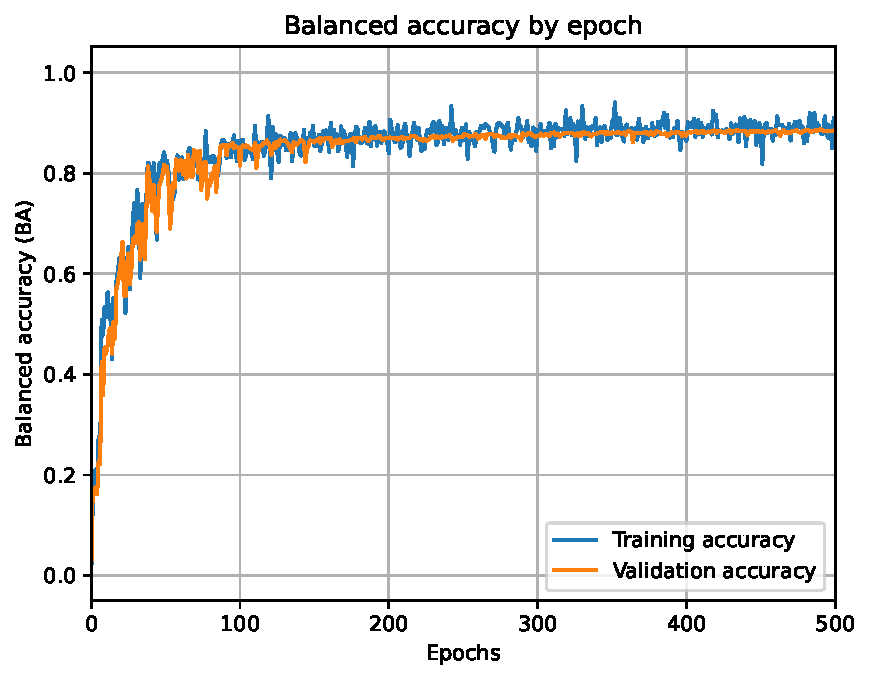
\includegraphics[width = \linewidth]{../../plot/LR_1/BA_500_epochs_batch_size500}
		\caption{Evolução da acurácia balanceada.}
		\label{fig:BA_500_epochs_batch_size500}
	\end{subfigure}
	\caption{Evolução da entropia cruzada e da acurácia balanceada durante o treinamento para \textit{mini-batch} de 500 amostras e $\eta = 0,01$.}
\end{figure}

Com o treinamento, obteve-se um classificador que ao aplicar os dados de teste, obteve uma acurácia balanceada média de 0,9162, com matriz de confusão mostrada na \autoref{tab:mc_lr_500} e métricas de precisão e \textit{recall} por classe listadas na \autoref{tab:pr_lr_500}. Observa-se facilmente o grande desempenho do classificador para a classe 6, possuindo total assertividade em identificar a classe, sem haver nenhum engano da classe com as outras, e vice-versa. Pela matriz, observa-se grande confusão da classe 1 com a classe 2 e 3, justificando a mesma possuir o menor \textit{recall}. Já a classe 3 é a que possuí menor precisão, sendo classificada erroneamente como a classe 1 e 2.

\begin{equation}\label{eq:ba_lr_500}
	BA = 0,9162
\end{equation}

\begin{table}[H]
	\centering
\begin{tabular}{c||c|c|c|c|c|c|}
	\cline{2-7}
	& \textbf{1} & \textbf{2} & \textbf{3} & \textbf{4} & \textbf{5} & \textbf{6} \\ \hline \hline
	\multicolumn{1}{|c||}{\textbf{1}} & 486        & 0          & 10         & 0          & 0          & 0          \\ \hline
	\multicolumn{1}{|c||}{\textbf{2}} & 30         & 440        & 1          & 0          & 0          & 0          \\ \hline
	\multicolumn{1}{|c||}{\textbf{3}} & 39         & 52         & 329        & 0          & 0          & 0          \\ \hline
	\multicolumn{1}{|c||}{\textbf{4}} & 0          & 3          & 0          & 424        & 64         & 0          \\ \hline
	\multicolumn{1}{|c||}{\textbf{5}} & 1          & 0          & 0          & 33         & 498        & 0          \\ \hline
	\multicolumn{1}{|c||}{\textbf{6}} & 0          & 0          & 0          & 0          & 0          & 537        \\ \hline
\end{tabular}
	\caption{Matriz de confusão do classificador com \textit{mini-batch} de 500 amostras.}
	\label{tab:mc_lr_500}
\end{table}

\begin{table}[H]
	\centering
	\begin{tabular}{c|c|c}
		\textbf{Classe} & \textbf{Precisão} & \textit{\textbf{Recall}} \\ \hline
		\textbf{1}      & 0.9798            & 0.8741                   \\
		\textbf{2}      & 0.9342            & 0.8889                   \\
		\textbf{3}      & 0.7833            & 0.9676                   \\
		\textbf{4}      & 0.8635            & 0.9278                   \\
		\textbf{5}      & 0.9361            & 0.8861                   \\
		\textbf{6}      & 1.0000            & 1.0000                  
	\end{tabular}
	\caption{Precisão e \textit{Recall} por classe do classificador com \textit{mini-batch} de 500 amostras por classe.}
	\label{tab:pr_lr_500}
\end{table}



\subsubsection*{\textit{Mini-batch} 1000 amostras}

Ao aumentar o tamanho de amostras por atualização da matriz de pesos, observa-se uma convergência mais suave e mais assertiva, apresentando uma curva de acurácia balanceada (\autoref{fig:BA_500_epochs_batch_size1000}) mais bem comportada, devido à apresentar uma maior média de amostras para formar uma iteração de $\+W$ pelo gradiente negativo da entropia cruzada (\autoref{fig:CE_500_epochs_batch_size1000}).

% TODO: \usepackage{graphicx} required
\begin{figure}[H]
	\begin{subfigure}[H]{0.49\textwidth}
		\centering
		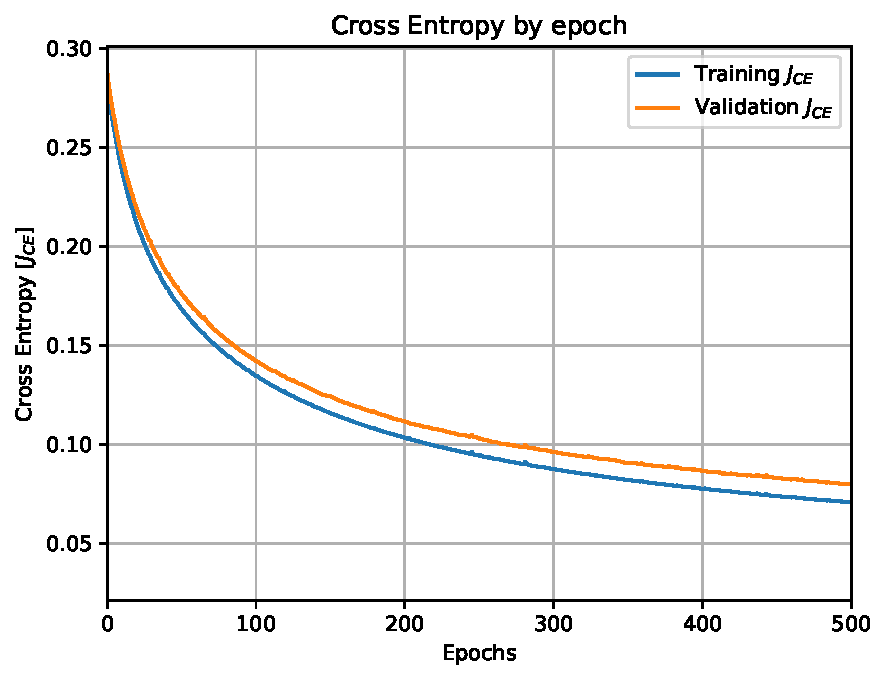
\includegraphics[width = \linewidth]{../../plot/LR_1/CE_500_epochs_batch_size1000}
		\caption{Evolução da entropia cruzada.}
		\label{fig:CE_500_epochs_batch_size1000}
	\end{subfigure}
	\begin{subfigure}[H]{0.49\textwidth}
		\centering
		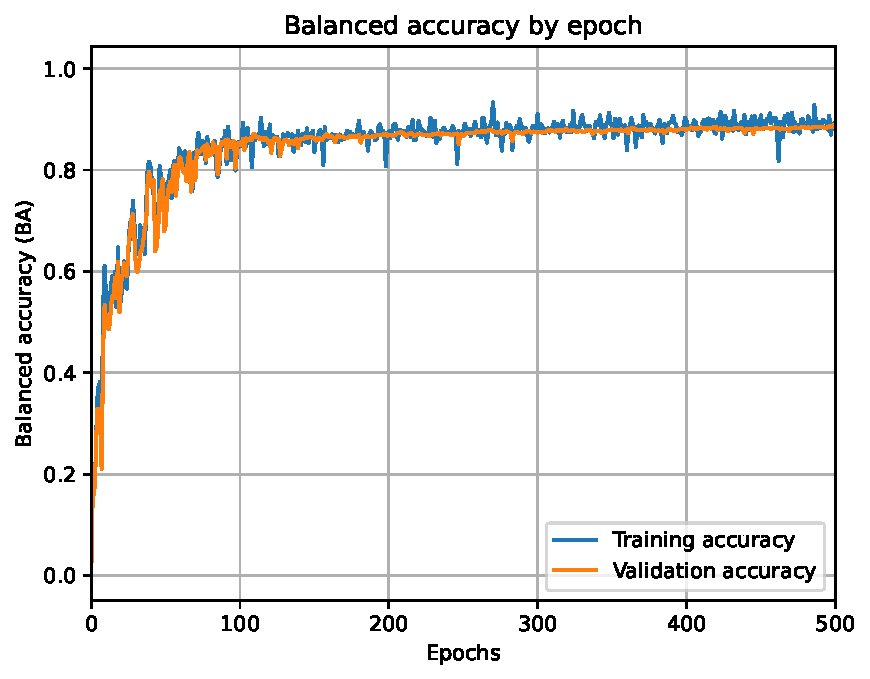
\includegraphics[width = \linewidth]{../../plot/LR_1/BA_500_epochs_batch_size1000}
		\caption{Evolução da acurácia balanceada.}
		\label{fig:BA_500_epochs_batch_size1000}
	\end{subfigure}
	\caption{Evolução da entropia cruzada e da acurácia balanceada durante o treinamento para \textit{mini-batch} de 1000 amostras e $\eta = 0,01$.}
\end{figure}

Com a alteração do tamanho da batelada utilizada, o modelo obteve um decrescimento no seu desempenho, atingindo uma acurácia balanceada de 0,9042. O comportamento da matriz de confusão (\autoref{tab:mc_lr_1000}) e das métricas de precisão e \textit{recall} (\autoref{tab:pr_lr_1000}) são similares, porém com menor desempenho comparados ao modelo anterior.

\begin{equation}\label{eq:ba_lr_1000}
BA = 0,9042
\end{equation}

\begin{table}[H]
\centering
\begin{tabular}{c||c|c|c|c|c|c|}
	\cline{2-7}
	& \textbf{1} & \textbf{2} & \textbf{3} & \textbf{4} & \textbf{5} & \textbf{6} \\ \hline\hline
	\multicolumn{1}{|c||}{\textbf{1}} & 486        & 0          & 10         & 0          & 0          & 0          \\ \hline
	\multicolumn{1}{|c||}{\textbf{2}} & 28         & 443        & 0          & 0          & 0          & 0          \\ \hline
	\multicolumn{1}{|c||}{\textbf{3}} & 56         & 53         & 311        & 0          & 0          & 0          \\ \hline
	\multicolumn{1}{|c||}{\textbf{4}} & 0          & 3          & 0          & 426        & 61         & 1          \\ \hline
	\multicolumn{1}{|c||}{\textbf{5}} & 0          & 1          & 0          & 54         & 477        & 0          \\ \hline
	\multicolumn{1}{|c||}{\textbf{6}} & 0          & 0          & 0          & 0          & 0          & 537        \\ \hline
\end{tabular}
\caption{Matriz de confusão do classificador com \textit{mini-batch} de 1000 amostras.}
\label{tab:mc_lr_1000}
\end{table}

\begin{table}[H]
\centering
\begin{tabular}{c|c|c}
	\textbf{Classe} & \textbf{Precisão} & \textit{\textbf{Recall}} \\ \hline
	\textbf{1}      & 0.9798            & 0.8526                   \\
	\textbf{2}      & 0.9406            & 0.8860                   \\
	\textbf{3}      & 0.7405            & 0.9688                   \\
	\textbf{4}      & 0.8676            & 0.8875                   \\
	\textbf{5}      & 0.8966            & 0.8866                   \\
	\textbf{6}      & 1.0000            & 0.9981                  
\end{tabular}
\caption{Precisão e \textit{Recall} por classe do classificador com \textit{mini-batch} de 1000 amostras por classe.}
\label{tab:pr_lr_1000}
\end{table}



\subsubsection*{\textit{Mini-batch} 2000 amostras}

Aumentando ainda mais o número de amostras por \textit{mini-batch}, observa-se uma envolução ainda mais comportada da acurácia balanceada, apresentando oscilações muito menos perceptíveis, como visto na \autoref{fig:BA_500_epochs_batch_size2000}. O decaimento da função de custo, \autoref{fig:CE_500_epochs_batch_size2000} se dá da mesma forma, uma vez que cada evolução do vetor de peso carrega a média da entropia cruzada para cada amostra da batelada.

O desempenho obtido ao utilizar 2000 amostras por \textit{mini-batch} é ainda menor, chegando a uma acurácia balanceada de 0,8898. A matriz de confusão, como pode ser observado na \autoref{tab:mc_lr_2000} e precisão e \textit{recall} das classes (\autoref{tab:pr_lr_2000}), se apresentam da mesma forma, onde mesmo com a queda de \textit{performance}, se observa o mesmo perfil de comportamento para as classes.

% TODO: \usepackage{graphicx} required
\begin{figure}[H]
	\begin{subfigure}[H]{0.49\textwidth}
		\centering
		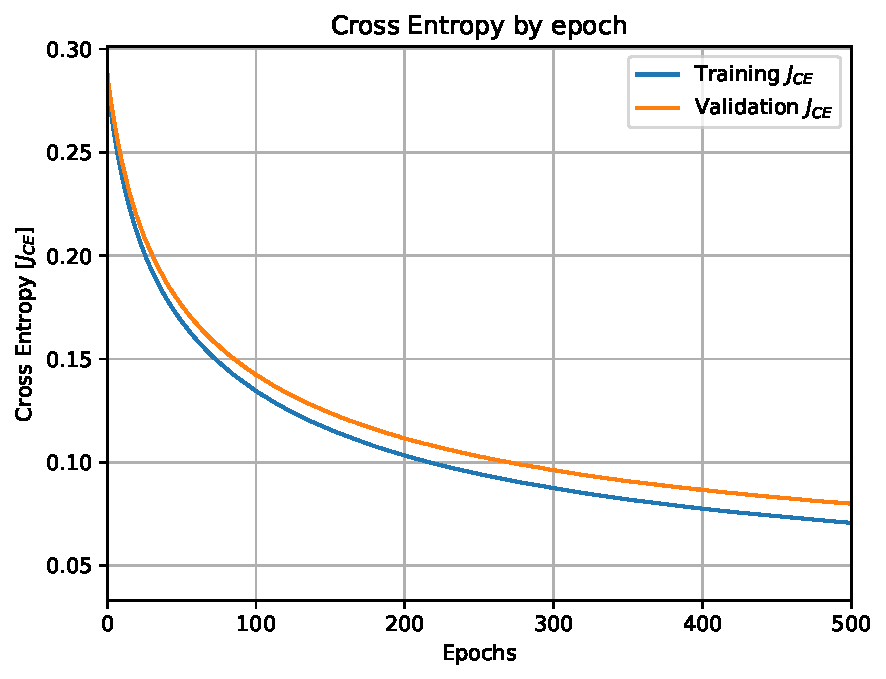
\includegraphics[width = \linewidth]{../../plot/LR_1/CE_500_epochs_batch_size2000}
		\caption{Evolução da entropia cruzada.}
		\label{fig:CE_500_epochs_batch_size2000}
	\end{subfigure}
	\begin{subfigure}[H]{0.49\textwidth}
		\centering
		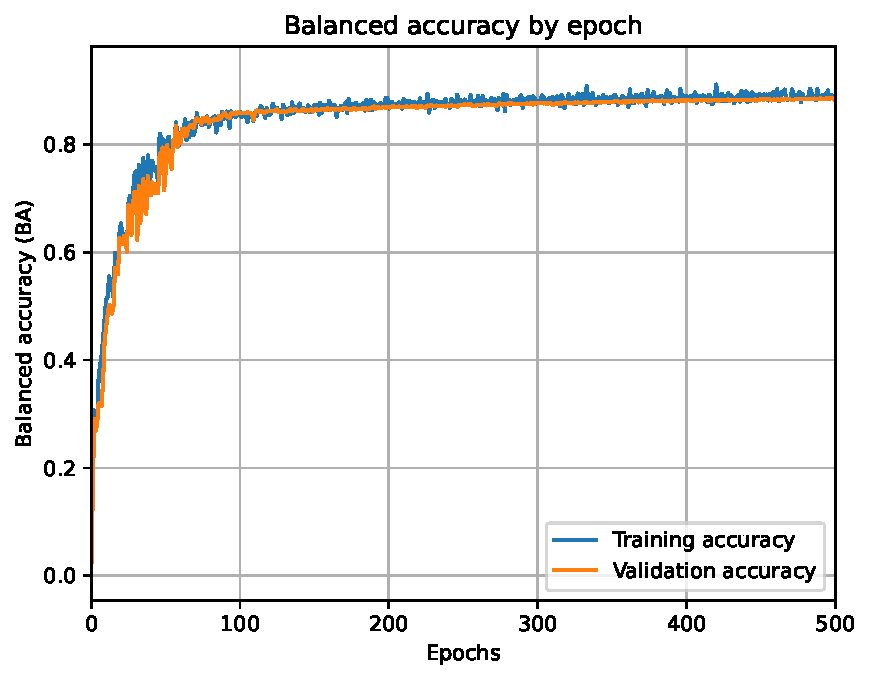
\includegraphics[width = \linewidth]{../../plot/LR_1/BA_500_epochs_batch_size2000}
		\caption{Evolução da acurácia balanceada.}
		\label{fig:BA_500_epochs_batch_size2000}
	\end{subfigure}
	\caption{Evolução da entropia cruzada e da acurácia balanceada durante o treinamento para \textit{mini-batch} de 2000 amostras e $\eta = 0,01$.}
\end{figure}

\begin{equation}\label{eq:ba_lr_2000}
BA = 0,8898
\end{equation}

\begin{table}[H]
\centering
\begin{tabular}{c||c|c|c|c|c|c|}
	\cline{2-7}
	& \textbf{1} & \textbf{2} & \textbf{3} & \textbf{4} & \textbf{5} & \textbf{6} \\ \hline\hline
	\multicolumn{1}{|c||}{\textbf{1}} & 489        & 0          & 7          & 0          & 0          & 0          \\ \hline
	\multicolumn{1}{|c||}{\textbf{2}} & 27         & 444        & 0          & 0          & 0          & 0          \\ \hline
	\multicolumn{1}{|c||}{\textbf{3}} & 70         & 49         & 301        & 0          & 0          & 0          \\ \hline
	\multicolumn{1}{|c||}{\textbf{4}} & 0          & 3          & 0          & 396        & 91         & 1          \\ \hline
	\multicolumn{1}{|c||}{\textbf{5}} & 1          & 1          & 0          & 58         & 472        & 0          \\ \hline
	\multicolumn{1}{|c||}{\textbf{6}} & 0          & 0          & 0          & 0          & 0          & 537        \\ \hline
\end{tabular}
\caption{Matriz de confusão do classificador com \textit{mini-batch} de 2000 amostras.}
\label{tab:mc_lr_2000}
\end{table}

\begin{table}[H]
\centering
\begin{tabular}{c|c|c}
	\textbf{Classe} & \textbf{Precisão} & \textit{\textbf{Recall}} \\ \hline
	\textbf{1}      & 0.9859            & 0.8330                   \\
	\textbf{2}      & 0.9427            & 0.8934                   \\
	\textbf{3}      & 0.7167            & 0.9773                   \\
	\textbf{4}      & 0.8065            & 0.8722                   \\
	\textbf{5}      & 0.8872            & 0.8384                   \\
	\textbf{6}      & 1.0000            & 0.9981                  
\end{tabular}
\caption{Precisão e \textit{Recall} por classe do classificador com \textit{mini-batch} de 2000 amostras .}
\label{tab:pr_lr_2000}
\end{table}

\subsubsection*{Análise do número de épocas de treinamento}

Foi realizado o treinamento do modelo para a \textit{mini-batch} de 500 amostras em um \textit{range} de 1000 épocas, para observar a acomodação da função de custo. Observa-se na \autoref{fig:CE_1000_epochs_batch_size500} que a taxa de decrescimento da entropia cruzada vai reduzindo, porém não chega a um estado de regime, também não obtendo o estado de \textit{overfitting} com o aumento do custo para a validação. É possível aferir também que não há grande aumento da acurácia balanceada, se fazendo então, o treinamento de 500 épocas feito anteriormente, suficiente para a obtenção de um modelo que explora de forma suficiente o espaço de hipóteses ($\mathcal{H}$).

\begin{figure}[H]
	\begin{subfigure}[H]{0.49\textwidth}
		\centering
		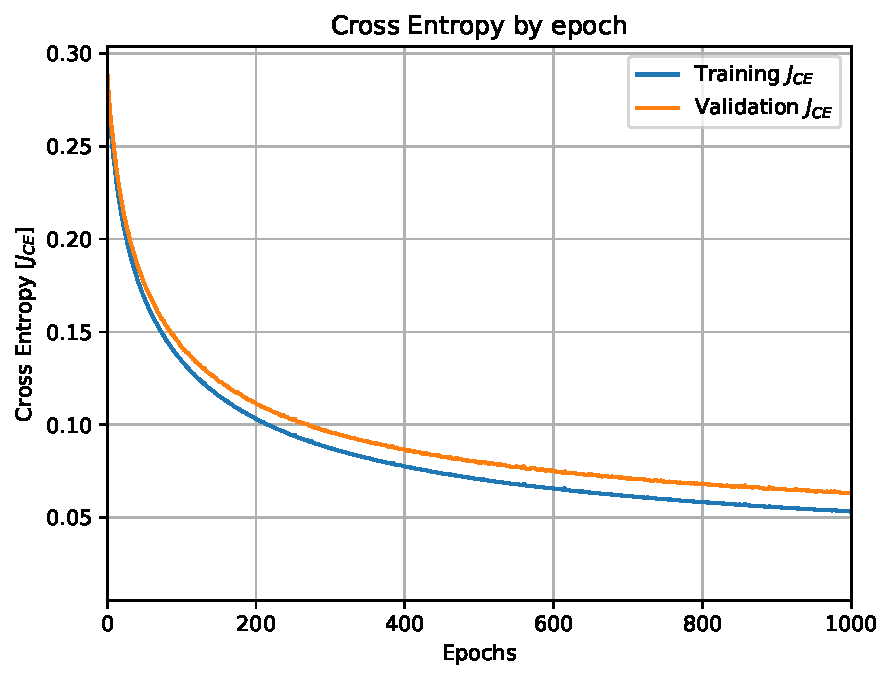
\includegraphics[width = \linewidth]{../../plot/LR_1/CE_1000_epochs_batch_size500}
		\caption{Evolução da entropia cruzada.}
		\label{fig:CE_1000_epochs_batch_size500}
	\end{subfigure}
	\begin{subfigure}[H]{0.49\textwidth}
		\centering
		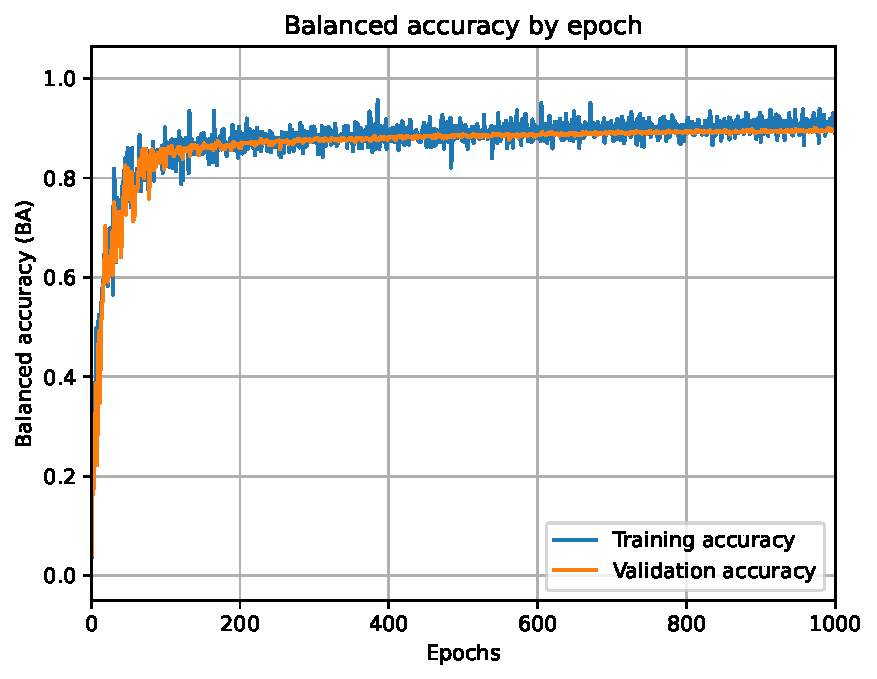
\includegraphics[width = \linewidth]{../../plot/LR_1/BA_1000_epochs_batch_size500}
		\caption{Evolução da acurácia balanceada.}
		\label{fig:BA_1000_epochs_batch_size500}
	\end{subfigure}
	\caption{Entropia cruzada e acurácia balanceada para o treinamento do modelo com \textit{mini-batch} de 500 amostras por 1000 épocas.}
\end{figure}





%%%%%%%%%%%%%%%%%%%%%%%%%%%%%%%%%%%%%%%%%%%%%%%%%%%%%%%%%%%
\subsection{Dados brutos}

%1) Organização dos dados
%2) Apresentação dos resultados
%3) Discussão das diferências

Considerando os hiper-parâmetros do melhor classificador utilizando a regressão logística testado com os dados pré-processados coletados do acelerômetro e do giroscópio, treinou-se um classificador para os dados brutos obtidos dos sensores. Esses dados possuem apenas as amostras de dados lidos dos sensores, ou seja, nenhuma informação útil é extraída \textit{a priori}.

A evolução da entropia cruzada e da acurácia balanceada para o treinamento utilizando \textit{mini-batch} de 500 amostras e passo $\eta = 0,01$ é mostrado na \autoref{fig:CE_BA_raw}. Rapidamente se observa a dificuldade em minimizar a função de custo, principalmente para os dados de validação, onde o decaimento da entropia cruzada é muito pequeno. Com a rápida saturação da entropia cruzada de validação, observa-se também a saturação da acurácia balanceada de validação, em um valor abaixo de 0,3, comprovando a dificuldade do modelo em reduzir o erro de classificação.

A acurácia balanceada do classificador após o treinamento é de 0,2506, apresentando um desempenho muito inferior ao classificador anterior treinado com dados tratados. A matriz de confusão da \autoref{tab:mc_lr_500_raw} comprova junto com o cálculo da precisão e \textit{recall} por classe (\autoref{tab:pr_lr_500_raw}), que o classificador apresenta uma enorme incapacidade de detectar certas classes, apresentando apenas 8 acertos para a classe 4. É interessante ressaltar que nessa situação, não se vê o mesmo comportamento do desempenho de classes visto anteriormente, onde a classe 3 que antes apresentava a pior precisão, agora apresenta a maior, pois com a mudança dos atributos, o modelo tenta aprender novas formas de relacionar os dados.

\begin{figure}[H]
	\begin{subfigure}[H]{0.49\textwidth}
		\centering
		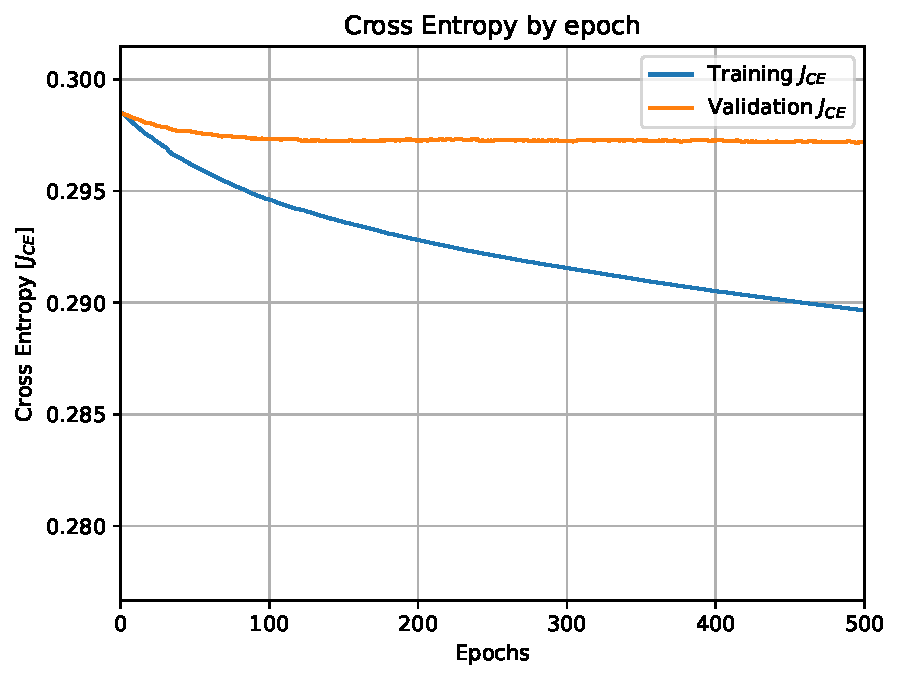
\includegraphics[width = \linewidth]{../../plot/LR_2/CE_500_epochs_batch_size500}
		\caption{Evolução da entropia cruzada.}
		\label{fig:CE_500_epochs_batch_size500_raw}
	\end{subfigure}
	\begin{subfigure}[H]{0.49\textwidth}
		\centering
		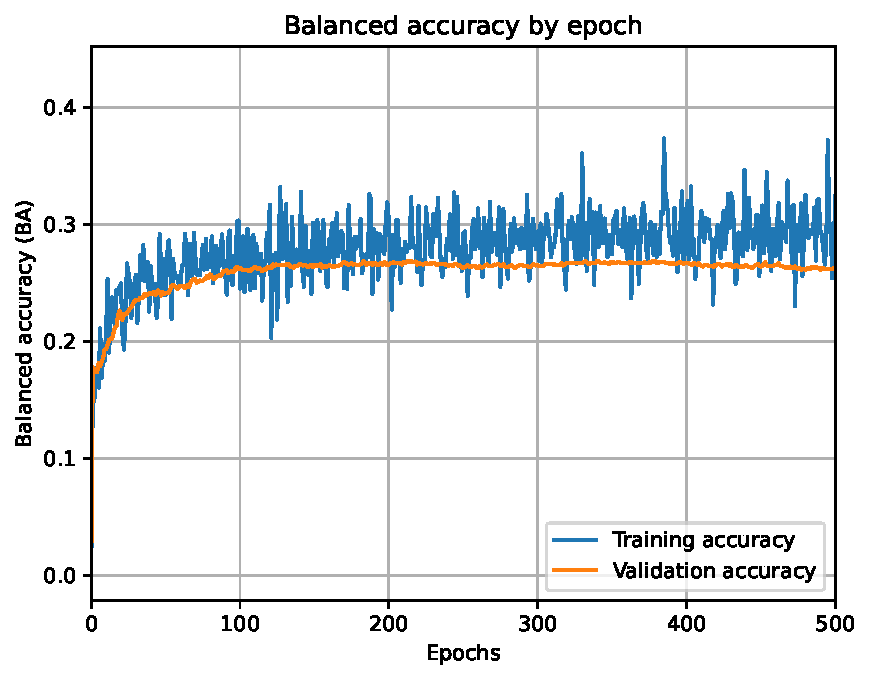
\includegraphics[width = \linewidth]{../../plot/LR_2/BA_500_epochs_batch_size500}
		\caption{Evolução da acurácia balanceada.}
		\label{fig:BA_500_epochs_batch_size500_raw}
	\end{subfigure}
	\caption{Entropia cruzada e acurácia balanceada para o treinamento do modelo com \textit{mini-batch} de 500 amostras por 500 épocas com dados brutos.}
	\label{fig:CE_BA_raw}
\end{figure}

\begin{equation}\label{eq:ba_lr_500_raw}
BA = 0,2506
\end{equation}

\begin{table}[H]
	\centering
\begin{tabular}{c||c|c|c|c|c|c|}
	\cline{2-7}
	\textbf{}                        & \textbf{1} & \textbf{2} & \textbf{3} & \textbf{4} & \textbf{5} & \textbf{6} \\ \hline \hline
	\multicolumn{1}{|c||}{\textbf{1}} & 99         & 177        & 149        & 13         & 19         & 39         \\ \hline
	\multicolumn{1}{|c||}{\textbf{2}} & 43         & 184        & 173        & 5          & 14         & 52         \\ \hline
	\multicolumn{1}{|c||}{\textbf{3}} & 17         & 127        & 228        & 16         & 12         & 20         \\ \hline
	\multicolumn{1}{|c||}{\textbf{4}} & 15         & 109        & 139        & 8          & 31         & 189        \\ \hline
	\multicolumn{1}{|c||}{\textbf{5}} & 31         & 163        & 165        & 9          & 34         & 130        \\ \hline
	\multicolumn{1}{|c||}{\textbf{6}} & 19         & 161        & 158        & 5          & 38         & 156        \\ \hline
\end{tabular}
	\caption{Matriz de confusão do classificador com \textit{mini-batch} de 500 amostras com dados brutos.}
	\label{tab:mc_lr_500_raw}
\end{table}

\begin{table}[H]
	\centering
\begin{tabular}{c|c|c}
	\textbf{Classe}     & \textbf{Precisão} & \textbf{\textit{Recall}} \\ \hline
	\textbf{1} & 0.1996            & 0.4420          \\
	\textbf{2} & 0.3907            & 0.1998          \\
	\textbf{3} & 0.5429            & 0.2253          \\
	\textbf{4} & 0.0163            & 0.1429          \\
	\textbf{5} & 0.0639            & 0.2297          \\
	\textbf{6} & 0.2905            & 0.2662          \\
\end{tabular}
	\caption{Precisão e \textit{Recall} por classe do classificador com \textit{mini-batch} de  500 amostras com dados brutos.}
	\label{tab:pr_lr_500_raw}
\end{table}



%%%%%%%%%%%%%%%%%%%%%%%%%%%%%%%%%%%%%%%%%%%%%%%%%%%%%%%%%%%
\clearpage
\section{Classificação via \textit{k neareast neighbours}}

A classificação pelo método \textit{k neareast neighbours} é baseada em inferir a classe do dado a ser classificado com base nos $k$ dados mais próximos à ele. Como hiper-parâmetros para esse problema, têm-se principalmente o valor de $k$, a ordem $p$ da distância de Minkowski entre os dados e o critério de classificação.

O critério de classificação pode se basear puramente na classe majoritária entre os $k$ vizinhos, ou levar em consideração a distância como um peso, que normalmente é inversamente proporcional a distância, evidenciando o rótulo dos pontos mais próximos do dado teste.


%%%%%%%%%%%%%%%%%%%%%%%%%%%%%%%%%%%%%%%%%%%%%%%%%%%%%%%%%%%
\subsection{Dados tratados}

Para implementação do algoritmo de \textit{k}-NN, foi escolhido a utilização da distância euclidiana no espaço dos atributos, e a decisão do rótulo vencedor por meio do voto majoritário dos $k$ vizinhos mais próximos.

Para obtenção do valor de $k$, foi executada uma busca em \textit{grid} do hiper-parâmetro, variando seu valor entre 1 e 29. Utilizando da técnica de validação cruzada \textit{k-fold}, com quatro pastas, foi realizada a inferência das classes dos dados da pasta de validação com base nos vizinhos mais próximos encontrados nas pastas de treinamento, para cada valor de $k$ testado. A \autoref{fig:gridsearch} exibe à evolução da acurácia balanceada para os valores de $k$, obtendo um conjunto de valores ótimos em \eqref{eq:k_fold_k}.

\begin{equation}\label{eq:k_fold_k}
	k = [17\ 28\ 12\ 18]
\end{equation}


% TODO: \usepackage{graphicx} required
\begin{figure}[H]
	\centering
	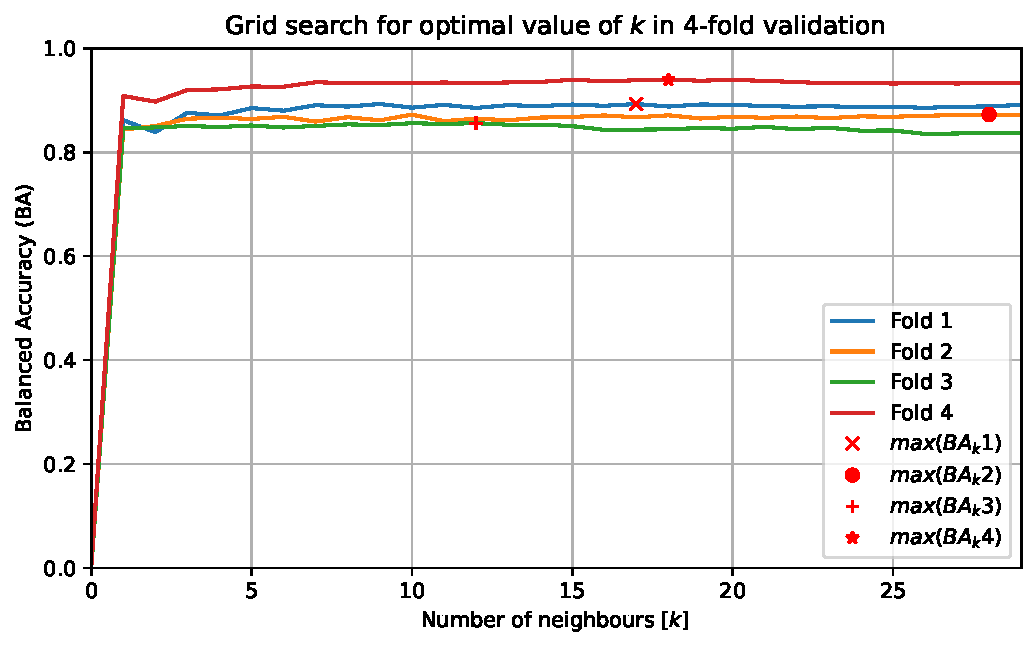
\includegraphics[width=0.75\linewidth]{../../plot/knn_1/grid_search_k_fold}
	\caption{Busca em \textit{grid} do valor de $k$ ótimo utilizando \textit{4-fold validation}.}
	\label{fig:gridsearch}
\end{figure}

A heurística escolhida para avaliar o melhor valor de $k$ com base no conjunto obtido por meio da busca em \textit{grid} com validação cruzada se dá em obter a acurácia balanceada média das pastas e obter o número de vizinhos que maximiza essa combinação das pastas. A \autoref{fig:gridsearch-k_optimal} mostra a progressão da acurácia balanceada média de acordo com $k$, e assim se obtém o valor de $k$ ótimo em $k = 15$.

\begin{figure}[H]
	\centering
	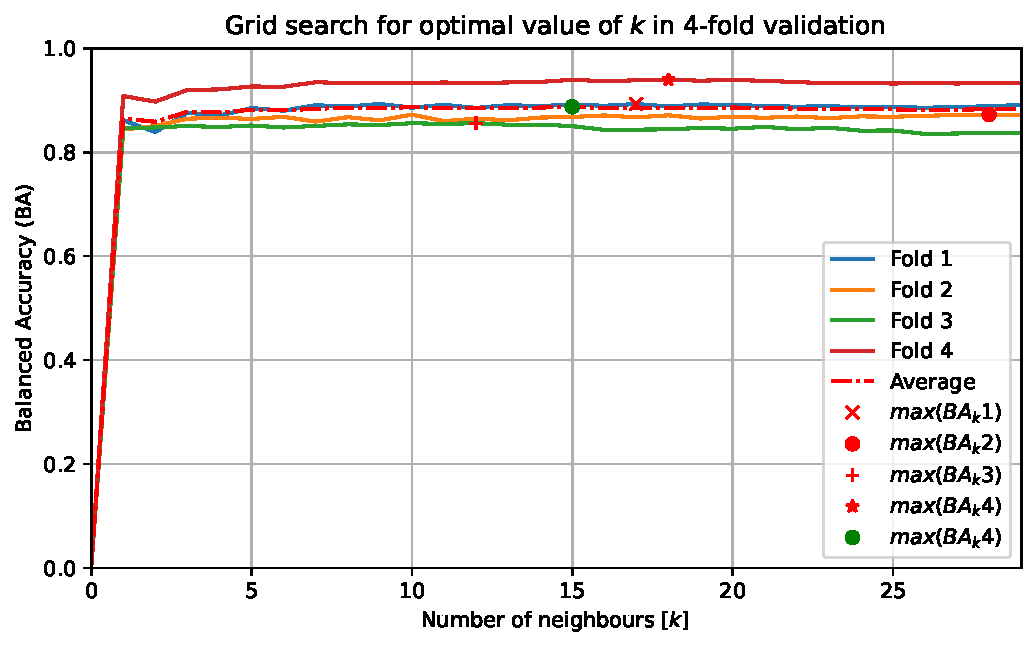
\includegraphics[width=0.75\linewidth]{../../plot/knn_1/grid_search_k_fold-k_optimal}
	\caption{Busca em \textit{grid} do valor de $k$ ótimo utilizando \textit{4-fold validation}.}
	\label{fig:gridsearch-k_optimal}
\end{figure}



Uma vez definido o classificador ótimo, obtém-se os indicadores de performance do classificador com base nos dados de teste. A acurácia balanceada encontrada foi de 0,8991 e a matriz de confusão do classificador por ser vista na \autoref{tab:mc_knn_1}.

\begin{equation}\label{eq:ba_knn_1}
	BA = 0,8991
\end{equation}

\begin{table}[H]
	\centering
	\begin{tabular}{c||c|c|c|c|c|c|}
		\cline{2-7}
		& \textbf{1} & \textbf{2} & \textbf{3} & \textbf{4} & \textbf{5} & \multicolumn{1}{l|}{\textbf{6}} \\ \hline \hline
		\multicolumn{1}{|c||}{\textbf{1}} & 488 & 0   & 8   & 0   & 0   & 0   \\ \hline
		\multicolumn{1}{|c||}{\textbf{2}} & 39  & 427 & 5   & 0   & 0   & 0   \\ \hline
		\multicolumn{1}{|c||}{\textbf{3}} & 51  & 44  & 325 & 0   & 0   & 0   \\ \hline
		\multicolumn{1}{|c||}{\textbf{4}} & 0   & 4   & 0   & 389 & 98  & 0   \\ \hline
		\multicolumn{1}{|c||}{\textbf{5}} & 0   & 0   & 0   & 31  & 501 & 0   \\ \hline
		\multicolumn{1}{|c||}{\textbf{6}} & 0   & 0   & 0   & 1   & 1   & 535 \\ \hline
	\end{tabular}
	\caption{Matriz de confusão do classificador \textit{k}-NN com \textit{k} = 15.}
	\label{tab:mc_knn_1}
\end{table}

Extraindo da matriz de confusão as métricas de precisão e \textit{recall}, obtém-se a \autoref{tab:pr_knn_1}. Pode-se observar que a classe 3 foi a que apresentou menor precisão, sendo muito confundida com a classe 1 e 2. Já a classe 1 possuí o pior \textit{recall}, uma vez que as classes 2 e 3 se confundem com a 1. A classe 6 foi a que apresentou o melhor desempenho, apresentando \textit{recall} unitário, logo, nenhuma classe se confunde com ela, e a maior precisão, muito próxima de 1.


\begin{table}[H]
	\centering
	\begin{tabular}{c|c|c}
		\textbf{Classe} & \textbf{Precisão} & \textbf{\textit{Recall}} \\ \hline
		\textbf{1}      & 0.9839 & 0.8443 \\
		\textbf{2}      & 0.9066 & 0.8989 \\
		\textbf{3}      & 0.7738 & 0.9615 \\
		\textbf{4}      & 0.7923 & 0.9240 \\
		\textbf{5}      & 0.9417 & 0.8350 \\
		\textbf{6}      & 0.9963 & 1.0000
	\end{tabular}
	\caption{Precisão e \textit{Recall} por classe do classificador.}
	\label{tab:pr_knn_1}
\end{table}

\subsubsection*{Comparação com a regressão logística}

Ao comparar os classificadores utilizando a regressão logística e o k-NN, observa-se que a acurácia balanceada para a regressão logística de melhor desempenho foi superior, mas para ter uma comparação mais minuciosa entre os dois classificadores, deve-se analisar também suas matrizes de confusão. Comparando a precisão e o \textit{recall}, o desempenho das classes em \textit{ranking} se apresenta da mesma forma, porém, para a regressão logística a classe 6 conseguiu obter tanto precisão quanto \textit{recall} máximo.

A regressão logística apresentou um desempenho relativo 1,87\% maior que o k-NN para a acurácia balanceada, porém possuí uma complexidade muito maior. Para obter o modelo de regressão logística multi-classe com \textit{softmax}, é necessário realizar o treinamento do modelo, buscando variar os hiper-parâmetros para se conseguir o melhor desempenho. Essa etapa demanda de muito processamento, porém garante uma utilização do classificador mais leve, uma vez que é necessária apenas o vetor de pesos. Já o \textit{k}-NN, não demanda treinamento, sendo necessária apenas a inferência da classe com base nos vizinhos mais próximos, o que apesar de consumir armazenamento para manter o \textit{dataset}, não precisa de tanto processamento prévio, sendo uma solução simples e de rápida implementação. 

Porém, devido a busca em \textit{grid} utilizando a validação \textit{k-fold} para obter o melhor $k$ para os dados de treinamento, tal etapa demandou bastante processamento, o que elevou consideravelmente a complexidade do \textit{k}-NN. Em relação ao tempo para realizar a classificação, o \textit{k}-NN também apresentou um tempo maior em comparação à regressão logística, devido à necessidade de varrer todo o \textit{dataset} para obter os dados mais próximos. Por outro lado, para a solução iterativa, basta aplicar a função \textit{softmax} com os pesos obtidos no treinamento, o que apresenta um tempo de execução consideravelmente menor.

\subsubsection*{Comparação com o $k$ ótimo}

Somente a título de comparação, foi realizada a busca em \textit{grid} do melhor valor de $k$, utilizando os próprios dados de teste do problema. A \autoref{fig:gridsearchk} mostra a evolução da acurácia balanceada dos dados de teste para o aumento do número de vizinhos, chegando ao valor ótimo em $k = 8$, com $BA = 0,9028$. 

Em comparação com o número de vizinhos obtidos via validação em \textit{k}-pastas, observa-se que o número de vizinhos é perto da metade do obtido anteriormente, e apresentando uma performance melhor. Porém, ao se realizar uma busca de um hiper-parâmetro com métodos de busca em \textit{grid} utilizando validação cruzada, busca-se obter o melhor valor com base nos dados de treinamento, que são os únicos conhecidos na etapa de treinamento/modelagem do classificador. Espera-se que os dados de treinamento sejam suficiente para generalizar os dados como um todo, fazendo com que a solução ótima para o \textit{dataset} de treinamento tenda a ser a solução ótima para todos os dados inéditos que o modelo irá receber.

Dessa forma, mesmo o valor de $k$ tendo mudado consideravelmente, a acurácia não apresentou grandes mudanças, sendo ainda sim um bom modelo para conseguir fazer a classificação dos dados de teste.

\begin{figure}[H]
	\centering
	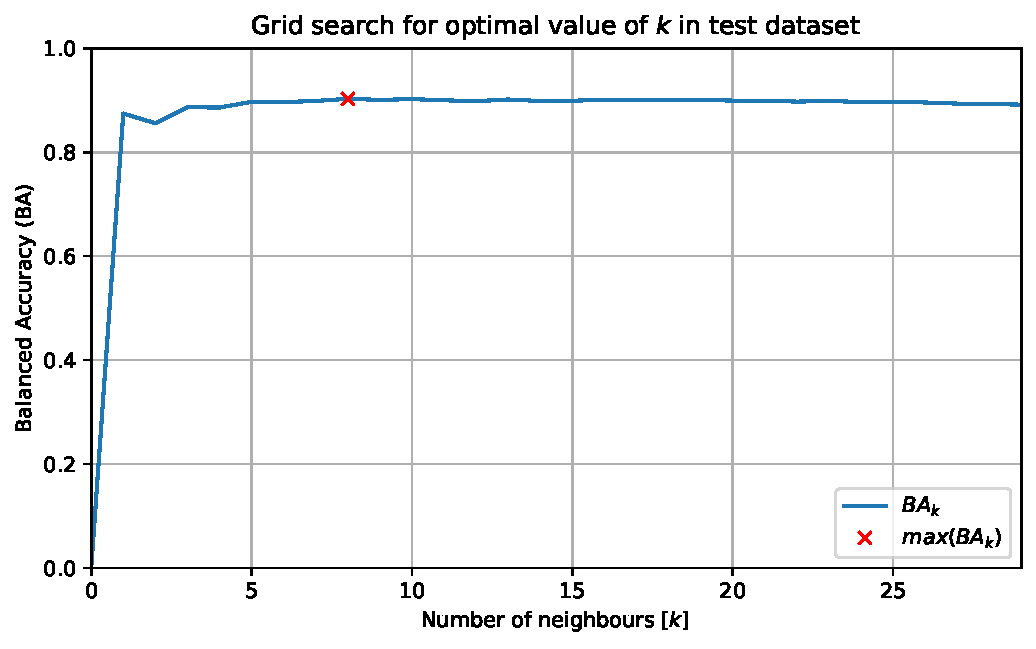
\includegraphics[width=0.75\linewidth]{../../plot/knn_1/grid_search}
	\caption{Busca em \textit{grid} do valor de $k$ ótimo para o conjunto de testes.}
	\label{fig:gridsearchk}
\end{figure}

%%%%%%%%%%%%%%%%%%%%%%%%%%%%%%%%%%%%%%%%%%%%%%%%%%%%%%%%%%%
\subsection{Dados brutos}

Utilizando agora para a aplicação do \textit{k}-NN o conjunto de dados brutos, formados pelos 768 atributos obtidos diretamente dos sensores para cada janela de tempo, realiza-se novamente a busca em \textit{grid} utilizando validação cruzada por meio da técnica \textit{k-fold} com 4 pastas. A \autoref{fig:gridsearch2} exibe a acurácia balanceada do classificador para o grupo de validação com cada uma das pastas de acordo com o aumento do número de vizinhos, onde foram obtidos os valores de $k$ ótimos para cada pasta de acordo com \eqref{eq:k_optimal2}.

\begin{equation}\label{eq:k_optimal2}
	k = [2\ 2\ 2\ 1]
\end{equation}

Adotando novamente a heurística de obter a acurácia balanceada média para todas as pastas, a \autoref{fig:gridsearch2} apresenta a curva dessa grandeza calculada na curva ponto-tracejada, e obtém-se que a métrica é maximizada por $k = 2$.


\begin{figure}[H]
	\centering
	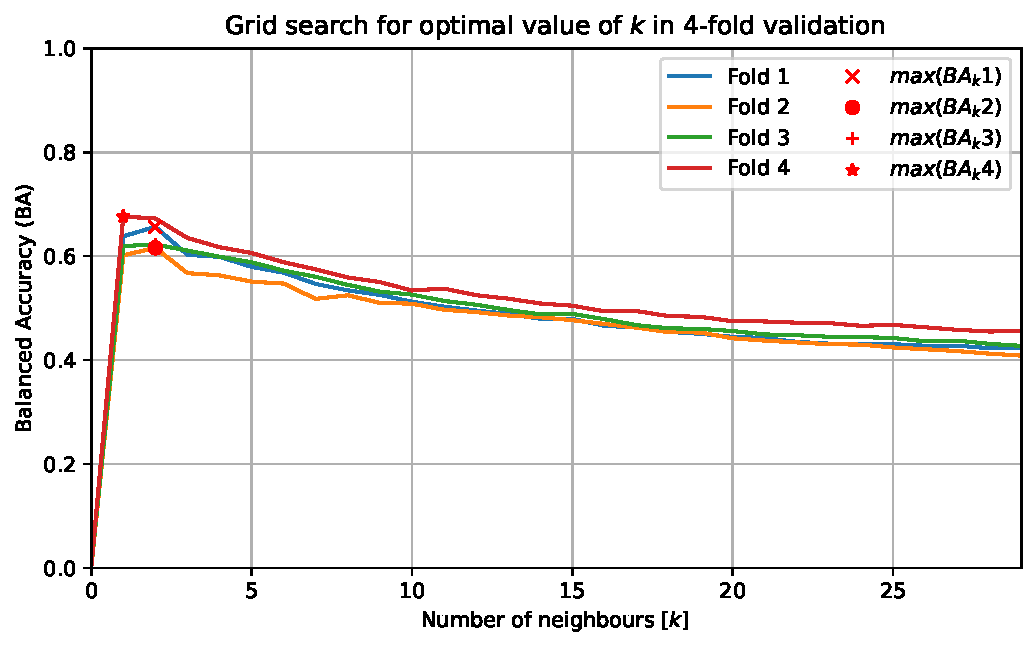
\includegraphics[width=0.75\linewidth]{../../plot/knn_2/grid_search_k_fold}
	\caption{Busca em \textit{grid} do valor de $k$ ótimo utilizando \textit{4-fold validation}.}
	\label{fig:gridsearch2}
\end{figure}

\begin{figure}[H]
	\centering
	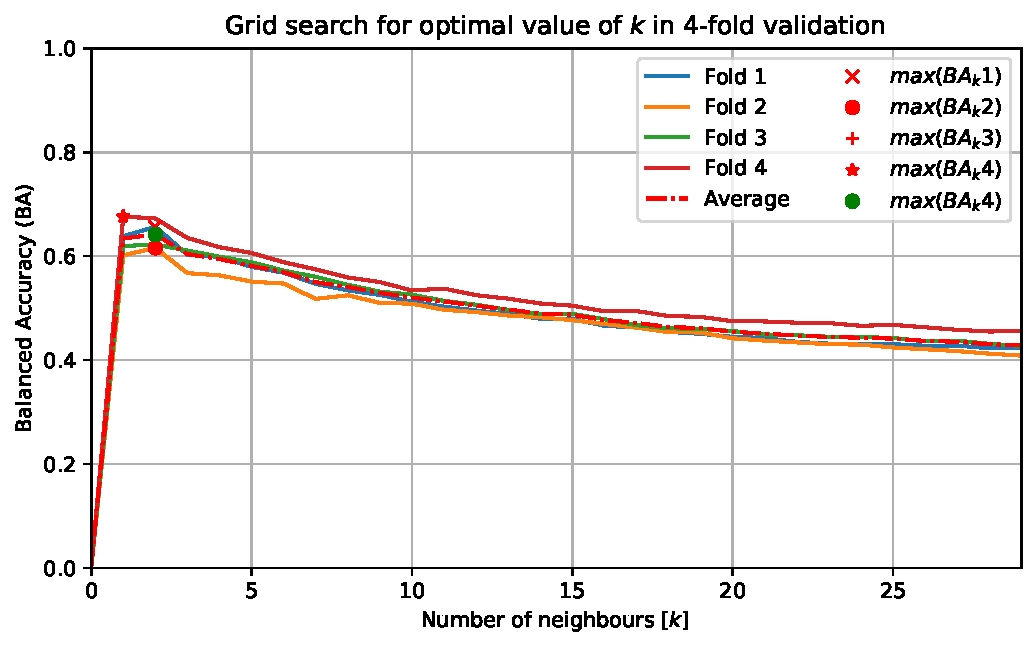
\includegraphics[width=0.75\linewidth]{../../plot/knn_2/grid_search_k_fold-k_optimal}
	\caption{Busca em \textit{grid} do valor de $k$ ótimo utilizando \textit{4-fold validation}.}
	\label{fig:gridsearch-k_optimal2}
\end{figure}

Realizando o teste do classificador obtido para o conjunto de dados brutos de teste, foi obtida uma acurácia balanceada que 0,6233, sendo sua matrix de confusão apresentada na \autoref{tab:mc_knn_2} e os valores de precisão e \textit{recall} na \autoref{tab:pr_knn_2}. Observa-se que a acurácia balanceada para dados brutos foi bem menor que utilizando o mesmo método para dados tratados, uma vez que existem menos informações extraídas para gerar vizinhos com informações de fácil comparação, tal resultado é esperado. Porém, o método de vizinhos mais próximos apresentou um resultado muito superior que a regressão logística para os dados brutos dos sensores, com mais que o dobro de acurácia.

\begin{equation}
	BA = 0.6233
\end{equation}

Observando a matrix de confusão (\autoref{tab:mc_knn_2}), é possível perceber que as classes 4, 5 e 6 não são confundidas com as classes 1, 2 e 3, porém são muito confundidas entre sí. Como essas classes representam o comportamento de estar de pé, sentado e deitado, espera-se que não haja movimento, ou seja, as leituras dos sensores para cada janela tendem a variar pouco, fazendo com que seja fácil diferenciar as classes que demandam movimento (caminhar, subir e descer escadas). Já as classes de movimento, essas se confundem com as classes que não possuem movimento, principalmente com a classe 5, que representa o estado de pé.

\begin{table}[H]
	\centering
	\begin{tabular}{c||c|c|c|c|c|c|}\cline{2-7}
\textbf{}                        & \textbf{1} & \textbf{2} & \textbf{3} & \textbf{4} & \textbf{5} & \textbf{6} \\ \hline \hline
\multicolumn{1}{|c||}{\textbf{1}} & 355        & 6          & 1          & 25         & 98         & 11         \\ \hline
\multicolumn{1}{|c||}{\textbf{2}} & 7          & 343        & 0          & 35         & 71         & 15         \\ \hline
\multicolumn{1}{|c||}{\textbf{3}} & 11         & 17         & 121        & 69         & 135        & 67         \\ \hline
\multicolumn{1}{|c||}{\textbf{4}} & 0          & 0          & 0          & 441        & 16         & 34         \\ \hline
\multicolumn{1}{|c||}{\textbf{5}} & 0          & 0          & 0          & 176        & 311        & 45         \\ \hline
\multicolumn{1}{|c||}{\textbf{6}} & 0          & 0          & 0          & 217        & 38         & 282        \\ \hline
\end{tabular}
	\caption{Matriz de confusão do classificador \textit{k}-NN com \textit{k} = 2 para dados brutos.}
	\label{tab:mc_knn_2}
\end{table}

Ao fornecer dados brutos para o classificador, o mesmo aprende como realizar a classificação por meio de características diferentes dos dados, ao se comparar com os dados tratados. Dessa forma, ao mudar os atributos e como eles são considerados, se observa que o comportamento do desempenho das classes muda consideravelmente, onde a classe 4, que para dados tratados apresentada a segunda pior precisão, agora apresenta a melhor. Já a classe 3, passou a apresentar o melhor \textit{recall}.

\begin{table}[H]
	\centering
	\begin{tabular}{c|c|c}
		\textbf{Classe} & \textbf{Precisão} & \textit{\textbf{Recall}} \\ \hline
		\textbf{1}      & 0.7157            & 0.9517                   \\
		\textbf{2}      & 0.7282            & 0.9372                   \\
		\textbf{3}      & 0.2881            & 0.9918                   \\
		\textbf{4}      & 0.8982            & 0.4579                   \\
		\textbf{5}      & 0.5846            & 0.4649                   \\
		\textbf{6}      & 0.5251            & 0.6211                  
	\end{tabular}
	\caption{Precisão e \textit{Recall} por classe do classificador para dados brutos.}
	\label{tab:pr_knn_2}
\end{table}

%%%%%%%%%%%%%%%%%%%%%%%%%%%%%%%%%%%%%%%%%%%%%%%%%%%%%%%%%%%
\clearpage
\section{Análise dos resultados}

%1) Classificador regressão logistica

	


%2) kNN




%3) Desempenho das classes



%4) Dados brutos vs dados processados

%	4.1) Dados com menos propriedades explicitas
%	4.2) São mais atributos, mas no fim das contas são 6 séries temporais de cada atributo
%	4.3) O modelo não tem capacidade de extrair atributos dos dados durante o treinamento,	
%		 logo pela sua simplicidade é necessário pré-processamento. Modelos como deep learning
%		 pela sua complexidade não precisam.




